\documentclass[tikz,border=4pt]{standalone}

\usepackage{amssymb}
\usetikzlibrary{arrows.meta,decorations.pathreplacing,positioning}

\begin{document}
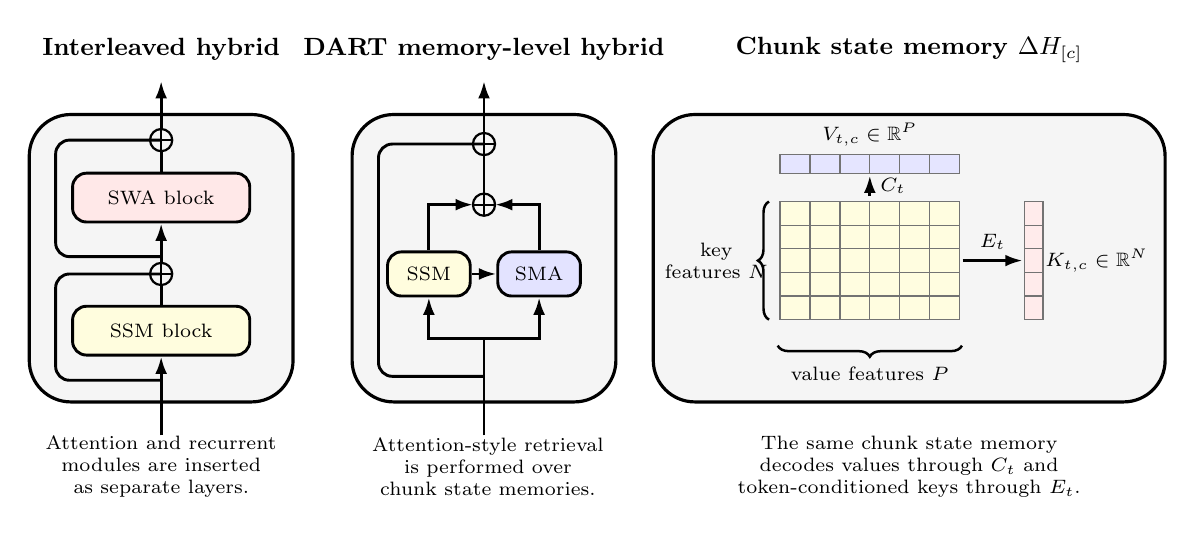
\begin{tikzpicture}[
    outer/.style={draw, fill=black!4, rounded corners=15pt, line width=1.15pt,
        minimum width=3.0cm, minimum height=3.05cm},
    block/.style={draw, rounded corners=5pt, line width=1.05pt, align=center,
        minimum width=2.25cm, minimum height=0.62cm,
        inner sep=3pt, font=\scriptsize},
    attn/.style={block, fill=red!9},
    ssm/.style={block, fill=yellow!13},
    sma/.style={block, fill=blue!11},
    residual/.style={line width=1.05pt, rounded corners=5pt},
    oplus/.style={
        draw=black, line width=0.8pt, circle, minimum size=8pt,
        inner sep=0pt, outer sep=0pt,
        path picture={
            \draw (path picture bounding box.center) -- ++(0.3cm,0)
                (path picture bounding box.center) -- ++(-0.3cm,0)
                (path picture bounding box.center) -- ++(0,0.3cm)
                (path picture bounding box.center) -- ++(0,-0.3cm);
        },
    },
    matcell/.style={draw=black!55, fill=yellow!12, line width=0.45pt,
        minimum width=0.38cm,
        minimum height=0.30cm, inner sep=0pt},
    vcell/.style={draw=black!55, fill=blue!10, line width=0.45pt,
        minimum width=0.38cm,
        minimum height=0.24cm, inner sep=0pt},
    kcell/.style={draw=black!55, fill=red!8, line width=0.45pt,
        minimum width=0.24cm,
        minimum height=0.30cm, inner sep=0pt},
    title/.style={font=\small\bfseries, align=center},
    note/.style={font=\scriptsize, align=center},
    arrow/.style={-{Latex[length=2.2mm, width=1.5mm]}, line width=1.05pt},
    looparrow/.style={-{Latex[length=2.2mm, width=1.5mm]}, line width=1.05pt},
    brace/.style={decorate, decoration={brace, amplitude=4pt}, line width=0.9pt}
]
    \node[title] at (0, 2.65) {Interleaved hybrid};
    \node[outer, minimum width=3.35cm, minimum height=3.65cm]
        (left_outer) at (0, 0) {};
    \node[ssm] (left_ssm) at (0, -0.92) {SSM block};
    \node[oplus] (left_ssm_add) at (0, -0.20) {};
    \node[attn] (left_swa) at (0, 0.77) {SWA block};
    \node[oplus] (left_swa_add) at (0, 1.50) {};
    % \node[note, left=0.18cm of left_outer] {$N/2\times$};
    \draw[arrow] (0, -2.25) -- (left_ssm.south);
    \draw[line width=1.05pt] (left_ssm.north) -- (left_ssm_add.south);
    \draw[arrow] (left_ssm_add.north) -- (left_swa.south);
    \draw[line width=1.05pt] (left_swa.north) -- (left_swa_add.south);
    \draw[arrow] (left_swa_add.north) -- (0, 2.25);
    \draw[residual] (0, -1.55)
        -- (-1.34, -1.55)
        -- (-1.34, -0.20)
        -- (left_ssm_add.center);
    \draw[residual] (0, 0.02)
        -- (-1.34, 0.02)
        -- (-1.34, 1.50)
        -- (left_swa_add.center);

    \node[title] at (4.1, 2.65) {DART memory-level hybrid};
    \node[outer, minimum width=3.35cm, minimum height=3.65cm]
        (right_outer) at (4.1, 0) {};
    \coordinate (right_split) at (4.1, -1.02);
    \node[ssm, minimum width=1.05cm, minimum height=0.56cm]
        (right_ssm) at (3.4, -0.20) {SSM};
    \node[sma, minimum width=1.05cm, minimum height=0.56cm]
        (right_sma) at (4.8, -0.20) {SMA};
    \node[oplus] (right_memory_add) at (4.1, 0.68) {};
    \node[oplus] (right_residual_add) at (4.1, 1.45) {};
    % \node[note, left=0.18cm of right_outer] {$N\times$};
    \draw[line width=1.05pt] (4.1, -2.25) -- (right_split);
    \draw[arrow] (right_split) -- (3.4, -1.02) -- (right_ssm.south);
    \draw[arrow] (right_split) -- (4.8, -1.02) -- (right_sma.south);
    \draw[arrow] (right_ssm.east) -- (right_sma.west);
    \draw[arrow] (right_ssm.north)
        -- (3.4, 0.68)
        -- (right_memory_add.west);
    \draw[arrow] (right_sma.north)
        -- (4.8, 0.68)
        -- (right_memory_add.east);
    \draw[line width=1.05pt]
        (right_memory_add.north) -- (right_residual_add.south);
    \draw[arrow] (right_residual_add.north) -- (4.1, 2.25);
    \draw[residual] (4.1, -1.50)
        -- (2.76, -1.50)
        -- (2.76, 1.45)
        -- (right_residual_add.center);

    \node[note, text width=3.15cm] at (0, -2.65)
        {Attention and recurrent modules are inserted as separate layers.};
    \node[note, text width=3.25cm] at (4.15, -2.65)
        {Attention-style retrieval is performed over chunk state memories.};

    \node[title] at (9.50, 2.65)
        {Chunk state memory $\Delta H_{[c]}$};
    \node[outer, minimum width=6.50cm, minimum height=3.65cm]
        (matrix_outer) at (9.50, 0) {};
    \foreach \c in {0,...,5} {
        \node[vcell] at (8.05 + 0.38*\c, 1.20) {};
    }
    \node[font=\scriptsize] at (9.0, 1.57)
        {$V_{t,c}\in\mathbb{R}^{P}$};

    \foreach \r in {0,...,4} {
        \foreach \c in {0,...,5} {
            \node[matcell] at (8.05 + 0.38*\c, 0.57 - 0.30*\r) {};
        }
    }
    \draw[decorate, decoration={brace, mirror, amplitude=4pt}, line width=0.9pt]
        (7.83, -1.11) --
        node[below=4pt, note] {value features $P$} (10.17, -1.11);
    \draw[decorate, decoration={brace, mirror, amplitude=4pt}, line width=0.9pt]
        (7.72, 0.72) -- (7.72, -0.78);
    \node[note, align=center] at (7.05, -0.03) {key\\features $N$};

    \draw[arrow] (9.0, 0.79) -- node[right, note] {$C_t$} (9.0, 1.05);

    \foreach \r in {0,...,4} {
        \node[kcell] at (11.08, 0.57 - 0.30*\r) {};
    }
    \node[font=\scriptsize] at (11.88, -0.03)
        {$K_{t,c}\in\mathbb{R}^{N}$};
    \draw[arrow] (10.18, -0.03) -- node[above, note] {$E_t$} (10.94, -0.03);

    \node[note, text width=4.5cm] at (9.50, -2.65)
        {The same chunk state memory decodes values through $C_t$ and
        token-conditioned keys through $E_t$.};
\end{tikzpicture}
\end{document}
